\documentclass{beamer}
\usetheme{metropolis}           % Use metropolis theme
\metroset{numbering=fraction}
\usepackage{tikz}
\usetikzlibrary{arrows,positioning,shapes.geometric}
\usepackage{float}
\usepackage{makecell}
\usepackage{fancyvrb}
\usepackage{listings}
\usepackage[export]{adjustbox}
\usepackage{caption}
\usepackage{alltt}
\title{Lecture 3 \\ More Java Basics}
\date{\today}
\author{Patrick Lam \\ Jeff Zarnett \\ Michael Giannikouris}
\institute{Department of Electrical and Computer Engineering}
\setbeamertemplate{caption}{\raggedright\insertcaption\par}
\setbeamersize{text margin left=12pt,text margin right=12pt}
\newcommand{\putat}[3]{\begin{picture}(0,0)(0,0)\put(#1,#2){#3}\end{picture}} % just a shorthand

\newenvironment{deflist}
{ \begin{description}
    \setlength{\itemsep}{6pt}
    \setlength{\parskip}{0pt}
    \setlength{\parsep}{0pt}     }
{ \end{description}              } 

\newenvironment{splitslide}
{
\centering
\begin{tabular}{@{}p{0.50\textwidth} | p{0.025\textwidth}@{} p{0.4\textwidth}@{}}
}
{
\end{tabular}
}


\begin{document}
\maketitle

\section{Java Arrays}

%%%%%%%%%%%%%%%%%%%%%%%%%%%%%%%%%%%%%%%%%%%%%%%%%%%%%%%%%%%%%%%%%%%%%%%%%%%%%%%%%%%%
% Arrays and Collections
%%%%%%%%%%%%%%%%%%%%%%%%%%%%%%%%%%%%%%%%%%%%%%%%%%%%%%%%%%%%%%%%%%%%%%%%%%%%%%%%%%%%
\begin{frame}{Arrays \& Collections}
The simple array is created with the \texttt{[]} square brackets. \\
\vspace{0.5em}
Example: \texttt{int[] numbers = new int[10];} \\
\vspace{0.5em}
You can have null elements in an array (say, of Strings) without this affecting the array length. \\
\vspace{0.5em}
An array is technically an object so you can assign it where a generic \texttt{Object} is expected. \\
\end{frame}
%%%%%%%%%%%%%%%%%%%%%%%%%%%%%%%%%%%%%%%%%%%%%%%%%%%%%%%%%%%%%%%%%%%%%%%%%%%%%%%%%%%%



%%%%%%%%%%%%%%%%%%%%%%%%%%%%%%%%%%%%%%%%%%%%%%%%%%%%%%%%%%%%%%%%%%%%%%%%%%%%%%%%%%%%
% Arrays
%%%%%%%%%%%%%%%%%%%%%%%%%%%%%%%%%%%%%%%%%%%%%%%%%%%%%%%%%%%%%%%%%%%%%%%%%%%%%%%%%%%%
\begin{frame}{Arrays}
Multidimensional arrays are also allowed, but only for primitive types \\
\vspace{1em}
\texttt{int[][][]  coordinates = new int[5][10][2];}.  \\
\vspace{1em}
This is not a big restriction since you can just have an array of arrays. \\
\vspace{1em}
Unlike some languages (C\#), you can't specify a rectangular array. \\
\end{frame}
%%%%%%%%%%%%%%%%%%%%%%%%%%%%%%%%%%%%%%%%%%%%%%%%%%%%%%%%%%%%%%%%%%%%%%%%%%%%%%%%%%%%



%%%%%%%%%%%%%%%%%%%%%%%%%%%%%%%%%%%%%%%%%%%%%%%%%%%%%%%%%%%%%%%%%%%%%%%%%%%%%%%%%%%%
% Arrays
%%%%%%%%%%%%%%%%%%%%%%%%%%%%%%%%%%%%%%%%%%%%%%%%%%%%%%%%%%%%%%%%%%%%%%%%%%%%%%%%%%%%
\begin{frame}{Arrays}
This is great, but like \texttt{String} an explicit array has a fixed size. \\
\vspace{0.5em}
What if we don't know how many element we need at compile time? \\
\vspace{0.5em}
\begin{itemize}
\item Create a new, bigger array and copy all the data?  \\
\item Allocate a very large array (i.e. 1000 elements) upfront? \\
\end{itemize}
\vspace{0.5em}
Wouldn't it be nice if we had a \textbf{dynamic} collection? \\
\end{frame}
%%%%%%%%%%%%%%%%%%%%%%%%%%%%%%%%%%%%%%%%%%%%%%%%%%%%%%%%%%%%%%%%%%%%%%%%%%%%%%%%%%%%



%%%%%%%%%%%%%%%%%%%%%%%%%%%%%%%%%%%%%%%%%%%%%%%%%%%%%%%%%%%%%%%%%%%%%%%%%%%%%%%%%%%%
% Java Collections
%%%%%%%%%%%%%%%%%%%%%%%%%%%%%%%%%%%%%%%%%%%%%%%%%%%%%%%%%%%%%%%%%%%%%%%%%%%%%%%%%%%%
\begin{frame}{Java Collections}
In Java, we do, and they're called, \texttt{Collection}s. \\
\vspace{1em}
The most common one: the \texttt{List}.  \\
\vspace{1em}
The type List takes a parameter in angle brackets to tell you what this is a list of. \\
\vspace{1em}
Example: \texttt{List<String>}. \\
\end{frame}
%%%%%%%%%%%%%%%%%%%%%%%%%%%%%%%%%%%%%%%%%%%%%%%%%%%%%%%%%%%%%%%%%%%%%%%%%%%%%%%%%%%%



%%%%%%%%%%%%%%%%%%%%%%%%%%%%%%%%%%%%%%%%%%%%%%%%%%%%%%%%%%%%%%%%%%%%%%%%%%%%%%%%%%%%
% Lists
%%%%%%%%%%%%%%%%%%%%%%%%%%%%%%%%%%%%%%%%%%%%%%%%%%%%%%%%%%%%%%%%%%%%%%%%%%%%%%%%%%%%
\begin{frame}{Lists}
Note that you can't call \texttt{new List<String>()} because no constructor exists for just plain \texttt{List}. \\
\vspace{1em}
Be specific about what kind of list you want to have, such as \texttt{ArrayList} (a very common one) or \texttt{LinkedList}. \\
\end{frame}
%%%%%%%%%%%%%%%%%%%%%%%%%%%%%%%%%%%%%%%%%%%%%%%%%%%%%%%%%%%%%%%%%%%%%%%%%%%%%%%%%%%%



%%%%%%%%%%%%%%%%%%%%%%%%%%%%%%%%%%%%%%%%%%%%%%%%%%%%%%%%%%%%%%%%%%%%%%%%%%%%%%%%%%%%
% Three Basic Collections
%%%%%%%%%%%%%%%%%%%%%%%%%%%%%%%%%%%%%%%%%%%%%%%%%%%%%%%%%%%%%%%%%%%%%%%%%%%%%%%%%%%%
\begin{frame}{Three Basic Collections}
Three basic collections exist: \\
\vspace{0.5em}
\begin{enumerate}
	\item List
	\item Map (in a later lecture)
	\item Set (like a list, but no duplicates)
\end{enumerate}
\end{frame}
%%%%%%%%%%%%%%%%%%%%%%%%%%%%%%%%%%%%%%%%%%%%%%%%%%%%%%%%%%%%%%%%%%%%%%%%%%%%%%%%%%%%



\begin{frame}{\texttt{static}}
When you see the keyword \texttt{static}, it is a modifier that means there is only one copy of the thing. 

\texttt{main()} in Java is declared as \texttt{static}; \\
\quad declare variables as \texttt{static} to reference them in \texttt{main}. 

Let's examine the semantics of this keyword.
\end{frame}

\begin{frame}{Static Variable}

The variable is common to all instances of a class. 

Assume you have an integer \texttt{i} in class $A$ and there are two instances of the class called $A_{1}$ and $A_{2}$. 

The value of \texttt{i} is the same and shared between $A_{1}$ and $A_{2}$.

A common variable can  keep a running total of the number of times a method has been called.

\end{frame}

\begin{frame}{Static Method}
The method is shared between all instances of the class. 	\\
Cannot access instance variables/methods of the class.		\\
\quad only methods and variables that share the static modifier.
\end{frame}

\begin{frame}{Static Class}
The modifier cannot be applied to a class. 

There are a number of useful Java classes which offer their functionality only in \texttt{static} methods, such as the \texttt{Math} class. 

Using \texttt{Math} you can perform such operations as square root.

It doesn't make logical sense to instantiate \texttt{new Math()} to perform such an operation. 
\end{frame}



\begin{frame}{\texttt{final}}
Another keyword: \texttt{final}. This can be applied to three things, with slightly different meanings:
\begin{itemize}
	\item Field
	\item Method
	\item Class
\end{itemize}
\end{frame}



\begin{frame}{Interfaces}
\only<1>{One of these things is not like the others:}
\only<2>{All but one of these things implement the {\tt HasHandle} interface.}
\begin{center}
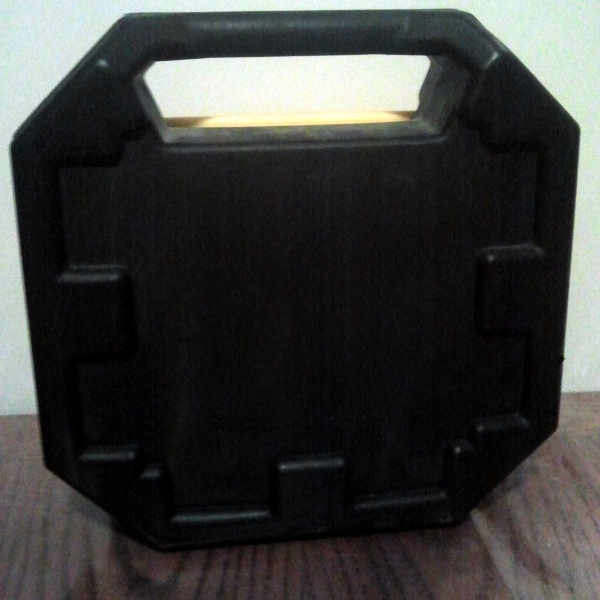
\includegraphics[width=.31\textwidth]{img/box-scaled.jpg}
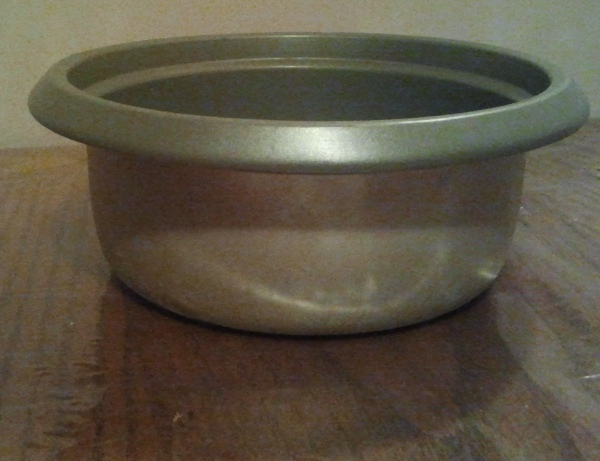
\includegraphics[width=.4\textwidth]{img/bowl-scaled.jpg}\\
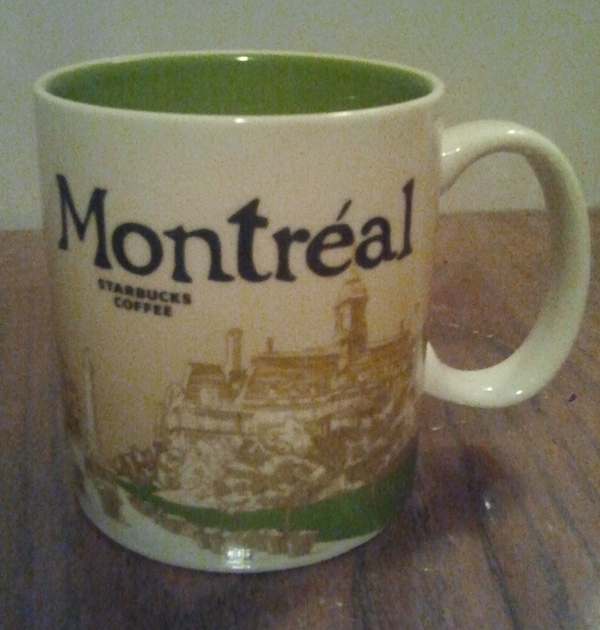
\includegraphics[width=.3\textwidth]{img/mug-scaled}
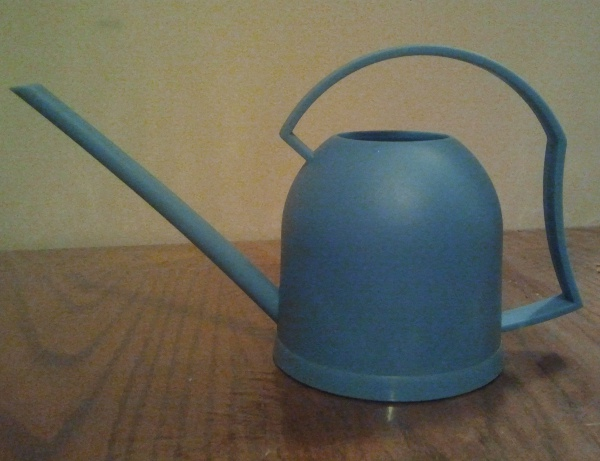
\includegraphics[width=.41\textwidth]{img/wateringcan-scaled.jpg}
\end{center}
\end{frame}



\begin{frame}{Using Interfaces}
\begin{alltt}
  interface HasHandle \{ \\
\qquad    void pickup(); \\
  \}\\[1em]
  class Donut \alert{implements} HasHandle \{ \\
\qquad    void pickup() \{ \ldots~\}  \\
\qquad    \ldots \\
  \}\\
\end{alltt}
\end{frame}



\begin{frame}{Interfaces as Contracts}
An \texttt{interface} is a way of specifying in Java what is effectively a contract. 

The interface specifies some number of methods which any class that wants to implement this interface must have.
\end{frame}


\begin{frame}[fragile]{Interfaces as Contracts}
\begin{verbatim}
public interface Drawable {
  void draw();
}
\end{verbatim}

Any class which implements \texttt{Drawable} must contain an implementation of the method \texttt{draw()}.
\end{frame}




\begin{frame}{Interface Semantics}
Methods that are declared in an interface are always public.\\
\quad Other modifiers are not allowed.

Interfaces can extend other interfaces, but may never contain implementation. 

An interface may declare some constants.

Accordingly, an interface can never be instantiated. 

A class can implement as many interfaces as desired.

We cannot apply the \texttt{final} keyword to an interface class, because we obviously have to implement it somehow.
\end{frame}





\begin{frame}{Why Interfaces?}
Interact with an object without knowing what it is underneath. 

Example: \texttt{Comparable} allows the JRE to sort objects.

For a built-in sort, the object must implement \texttt{Comparable}.\\\quad (otherwise Java has no idea how to order them). 

\texttt{Comparable}: only one method (\texttt{CompareTo}) is required.
\end{frame}





\begin{frame}{Why Interfaces?}
 If the objects we are looking at represent soccer players. 
 
 Sort them by their uniform numbers ascending. 
 
 Implement that logic in \texttt{CompareTo}. 
 
 Then we can use something like \texttt{Collections.sort()}. 
 
 The JRE sorts without having to know anything in advance about the soccer players.
\end{frame}





\begin{frame}{Abstract Classes}
Halfway between an interface and a regular class is the \alert{abstract class}. 

Declared using the \texttt{abstract} keyword. 

May (but does not have to) contain abstract methods. 

However, any class that contains methods marked \texttt{abstract} must also be marked as \texttt{abstract}. 

Cannot be instantiated, but may be subclassed. 

We cannot apply the \texttt{final} keyword to an abstract class, because it's meant to be subclassed.

An abstract class can have as much or as little implementation as desired.
\end{frame}





\begin{frame}[fragile]{Abstract Classes}
To declare an abstract method, write the method signature, but with the keyword \texttt{abstract} attached: 

\verb+public abstract void draw(int parameter);+.

Abstract classes may have static fields and methods.\\
\quad e.g. \texttt{AbstractClass.method()}.
\end{frame}




\begin{frame}{Abstract Classes vs. Interfaces}
There are similarities between abstract classes \& interfaces.
When should each of these be used?
\end{frame}




\begin{frame}{Use Abstract Class When}
\begin{itemize}
\item To share code among several closely related classes.
\item Classes that extend your abstract class have many common methods or fields, or require access modifiers other than public (such as protected and private).
\item To declare non-static or non-final fields. 
\end{itemize}
\end{frame}




\begin{frame}{Use Interface When}
\begin{itemize}
\item Unrelated classes would implement your interface. 
\item You want to specify the behaviour of a particular data type, but not concerned about who implements its behaviour.
\item You want to take advantage of multiple inheritance of type (i.e. implement multiple interfaces on one class)
\end{itemize}
\end{frame}




\begin{frame}{Why Not Both?}
An interface can be partly implemented by an abstract class.
The concrete class that extends the abstract class is responsible for implementing any of the methods of the interface that its superclass does not. 
\end{frame}

\begin{frame}{Why Not Both?}
Imagine interface $K$ has 4 methods. 

There is an abstract class $L$ declared as \texttt{implements K}. 

Suppose $L$ implements 3 of the 4 methods of $K$. 

When a subclass $P$ of $L$ is declared, then $P$ must implement that method that $L$ did not (or else be abstract itself).

\end{frame}


\end{document}